% ============================================================================
% chapters/ch05a.tex
% Xi Yin, Aspects of Two-Dimensional Conformal Field Theories (PoS TASI2017) 中译
% 本片段：PDF 第 34--40 页（原书 p.33--39）
%   5. 刻画二维 CFT 的版图
%   5.1 束缚间隙
%   5.2 束缚谱函数（至 (5.22)）
% 译者：tr05a    体例：work/style_guide.md
% ============================================================================

\section{刻画二维 CFT 的版图}\label{sec:5}

\begin{keytakeaways}
  \item 核心物理图像：二维 CFT 的谱与 OPE 数据并非任意。幺正性、交叉对称性与模不变性联手，把它们限制成一片“版图”。
  \item 使用的数学工具：环面配分函数的模不变性给出线性泛函方法，配合半正定规划；谱函数方法则把约束写成 Hilbert 空间中的完备性问题。
  \item 本节结论：模不变性给出维数间隙的界 $\Delta_{\mathrm{mod}}(c)$，而标量间隙界 $\Delta_{\mathrm{mod}}^{s=0}$ 在 $c=1,2,\frac{14}{5},4,8$ 处被能级 $1$ 的 WZW 模型饱和；谱函数方法把约束从间隙推广到整条谱。
\end{keytakeaways}

现在我们回到二维 CFT 的自举方法，从幺正性、交叉对称性与模不变性出发，考察一般的约束。

\subsection{束缚间隙}\label{sec:5-1}

先考察环面配分函数 \eqref{eq:3-48} 的模不变性给出的约束，其出发点只是系数 $d_{h,\tilde h}$ 的正性。设 $\alpha$ 是作用在 $\tau,\bar\tau$ 的函数空间上的任一线性泛函，模交叉方程 $Z(\tau,\bar\tau)=Z(-1/\tau,-1/\bar\tau)$ 便给出
\begin{equation}
  \label{eq:5-1}
  \sum_{h,\tilde h} d_{h,\tilde h}\,\alpha\bigl[\chi_h(\tau)\bar\chi_{\tilde h}(\bar\tau)
  -\chi_h(-1/\tau)\bar\chi_{\tilde h}(-1/\bar\tau)\bigr]=0 .
\end{equation}
% [Tutor Note: 这里取 $\tau\equiv ie^{z}$、$\bar\tau\equiv ie^{\bar z}$，模变换 $\tau\to-1/\tau$ 就是 $z\to-z$。因此方括号里的差只保留 $z,\bar z$ 展开中总阶数 $m+n$ 为奇数的项，这正是 (5.2) 求和限写 $m+n$ 为奇数的原因；若不理解这一点，会误以为 (5.2) 漏掉了偶数阶导数项。]
取 $\tau\equiv ie^{z}$、$\bar\tau\equiv ie^{\bar z}$，可把 $\alpha$ 在导数基上展开：
\begin{equation}
  \label{eq:5-2}
  \alpha=\sum_{m+n\ \text{odd}}\alpha_{m,n}\,\partial_z^m\partial_{\bar z}^n\big|_{z=\bar z=0} .
\end{equation}

给定一个假想的谱 $\mathcal{S}$。只要能找到 $\alpha$，使 $\alpha[\chi_h\bar\chi_{\tilde h}]\ge0$ 对所有 $(h,\tilde h)\in\mathcal{S}$ 成立，并且 $\alpha[\chi_0\bar\chi_0]>0$（此处假定单位算符属于算符谱），就与 \eqref{eq:5-1} 立刻矛盾，从而排除谱 $\mathcal{S}$。

举例来说，若 $\alpha[\chi_h\bar\chi_{\tilde h}]\ge0$ 对所有 $h+\tilde h>\Delta_0$ 成立，而在 $h=\tilde h=0$ 处取严格不等号，则可排除 Virasoro 原初场维数谱中存在间隙 $\Delta_0$ 的可能。

作为一个简单例子，考虑如下形式的线性泛函 \cite{r56}：
\begin{equation}
  \label{eq:5-3}
  \alpha=a_1(\partial_z+\partial_{\bar z})+a_3(\partial_z+\partial_{\bar z})^3\big|_{z=\bar z=0} .
\end{equation}
作替换
\begin{equation}
  \label{eq:5-4}
  \chi_h(\tau)\ \longrightarrow\ \hat\chi_h(\tau)=\tau^{\frac14}\eta(\tau)\chi_h(\tau).
\end{equation}
可以把模交叉方程略微化简。当 $c>1$ 时，$h>0$ 的 $\hat\chi_h(\tau)=\tau^{\frac14}q^{h-\frac{c-1}{24}}$；真空则为 $\hat\chi_0(\tau)=\tau^{\frac14}q^{-\frac{c-1}{24}}(1-q)$。为进一步简化，假定不存在任何自旋的守恒 Virasoro 原初流。于是直接计算得
\begin{equation}
  \label{eq:5-5}
  \alpha[\chi_h\bar\chi_{\tilde h}]
  =e^{-2\pi(\Delta-\frac{c-1}{12})}\bigl[a_1R_1(\Delta)+a_3R_3(\Delta)\bigr],
\end{equation}
对 $h,\tilde h>0$ 成立。这里 $R_n(\Delta)$ 是 $\Delta=h+\tilde h$ 的 $n$ 次多项式，其系数依赖 $c$ 与真空特征标：
\begin{equation}
  \label{eq:5-6}
  \begin{aligned}
  \alpha[\chi_0\bar\chi_0]={}&e^{2\pi\frac{c-1}{12}}\Bigl[a_1(-0.0118212+0.522621c)\\
  &\qquad +a_3(-0.245875-0.41425c+0.811209c^2+0.14328c^3)\Bigr].
  \end{aligned}
\end{equation}
% [Tutor Note: (5.5) 只对 $h,\tilde h>0$ 成立，而真空要单独用 (5.6) 处理，根源是 $\hat\chi_0\propto q^{-\frac{c-1}{24}}(1-q)$ 里那个 $(1-q)$ 因子：$h=0$ 时特征标不是纯幂次，展开会多出 $q$ 的整数次幂，从而给出一组纯数值的 $c$ 依赖系数。核对 (5.6) 时注意第二个方括号里 $c^3$ 项的符号为正。]
我们希望选取 $a_1,a_3$，使 \eqref{eq:5-6} 为正，且
\begin{equation}
  \label{eq:5-7}
  a_1R_1(x)+a_3R_3(x)\ge0\quad\forall x\ge\Delta_0,
\end{equation}
对某个 $\Delta_0$ 成立。这样的 $\Delta_0$ 就给出算符谱中间隙的上界。当 \eqref{eq:5-6} 取零、且 $a_3<0$ 时，$\Delta_0$ 达到最优（此处即取最小）；其值由 $a_1R_1(x)+a_3R_3(x)=0$ 的最大根给出。结果在大 $c$ 极限下可展开为
\begin{equation}
  \label{eq:5-8}
  \Delta_0\approx\frac{c}{6}+0.471824-0.03374\,c^{-1}+\mathcal{O}(c^{-2}) .
\end{equation}
% [Tutor Note: 注意 (5.8) 的常数项是 $0.471824$，而不是图 11 里 $c/6+1/3$ 的 $1/3$。原因很直接：只保留 $a_1,a_3$ 两项的泛函是一个受限子空间，(5.8) 得到的界比最优界更大（更弱）。$1/6$ 的首项系数则与图 11 中 $c/6+1/3$ 的斜率一致。]

在 $\alpha$ 中加入 $z,\bar z$ 的高阶导数可以改进这一结果 \cite{r57,r58}。例如，取形如 \eqref{eq:5-2} 的线性泛函并把求和截断到 $m+n\le N$，在这个泛函子空间里寻找最强的维数间隙界，记作 $\Delta_{\mathrm{mod}}^{(N)}$。再取极限 $N\to\infty$，得到维数间隙的最优模界 $\Delta_{\mathrm{mod}}=\lim_{N\to\infty}\Delta_{\mathrm{mod}}^{(N)}$。数值上，用 SDPB 程序包可以相当高效地算到 $N\approx55$；再对 $N$ 作数值外推，得到 $\Delta_{\mathrm{mod}}$ 作为中心荷 $c$ 的函数。结果见图~\ref{fig:11}。

\begin{figure}[htbp]
  \centering
  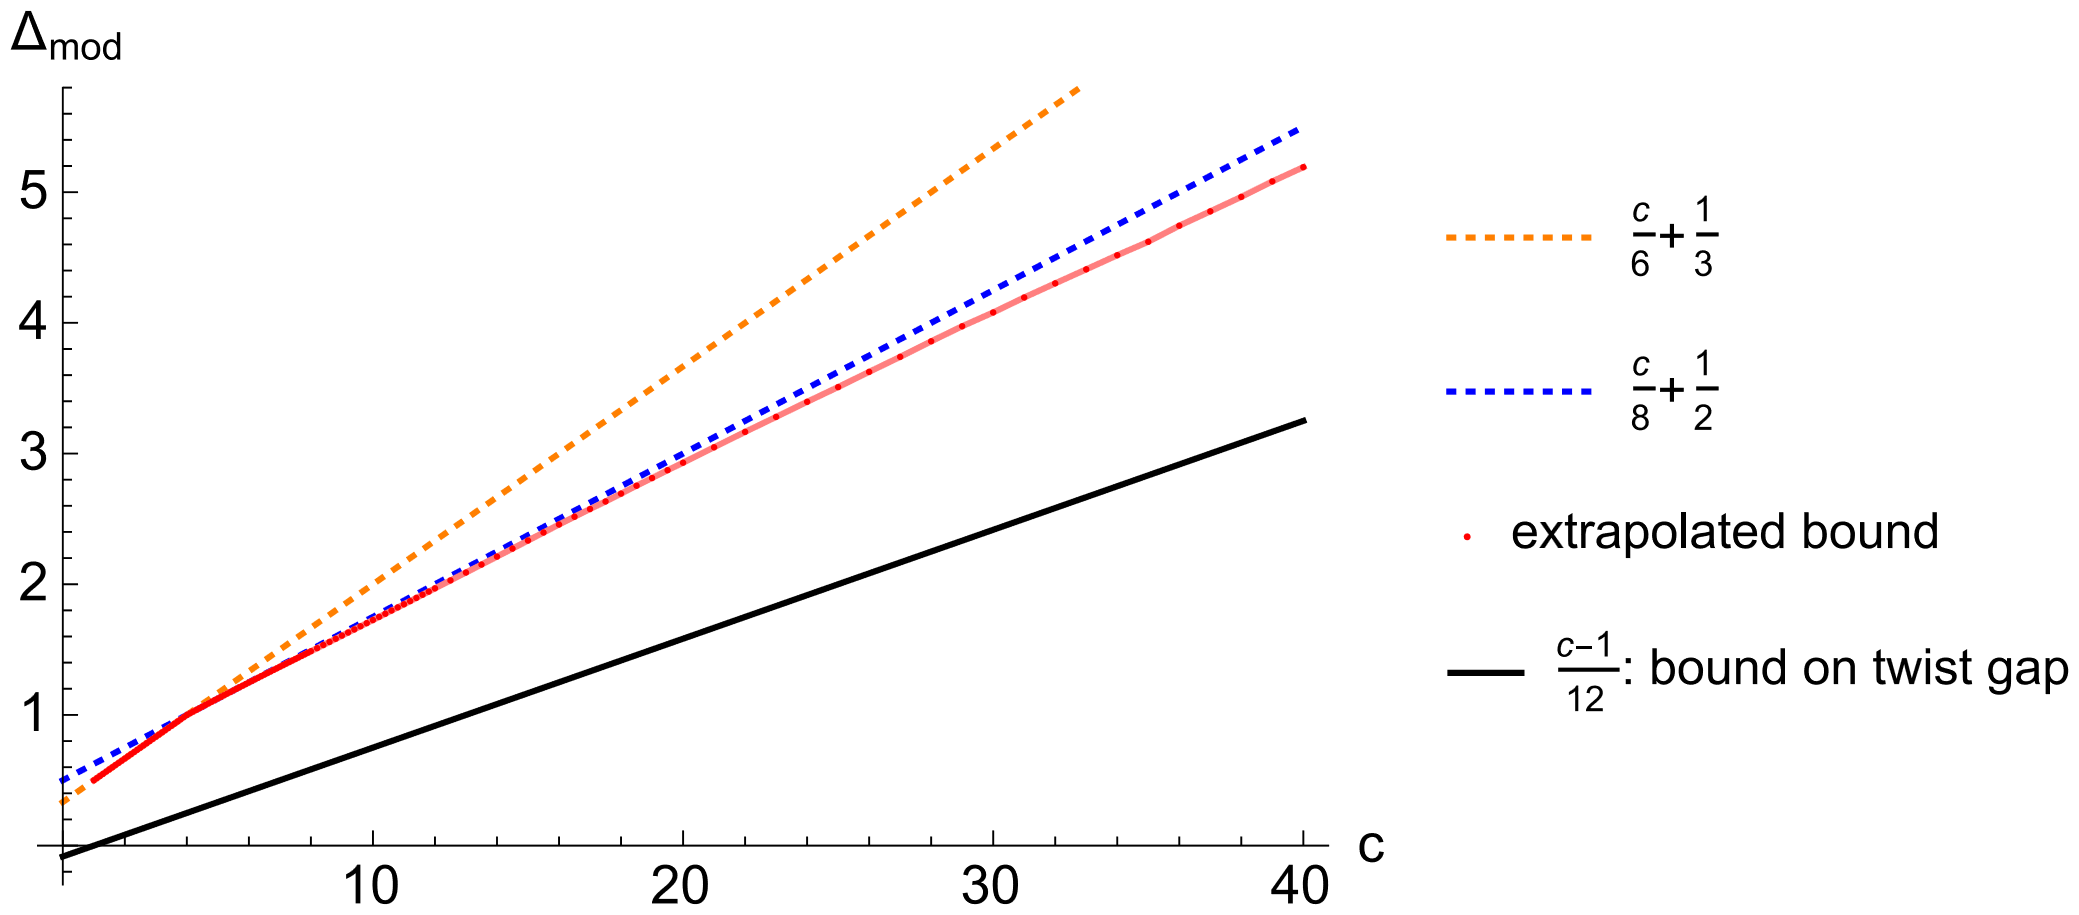
\includegraphics[width=0.85\textwidth]{figures/fig11.png}
  \caption{维数间隙的模界 $\Delta_{\mathrm{mod}}$（红色）作为中心荷 $c$ 的函数，由 $\Delta_{\mathrm{mod}}^{(N)}$ 数值外推到 $N=\infty$ 得到（用 $1/N$ 的二次多项式拟合 $31\le N\le55$ 的结果）\cite{r58}。（原文 p.35，图 11）}
  \label{fig:11}
\end{figure}

可以看到，对 $c\in[1,4]$，$\Delta_{\mathrm{mod}}(c)$ 恰等于 $\frac{c}{6}+\frac13$。它的斜率在 $c=4$ 处从 $\frac16$ 跳到 $\frac18$，此后随 $c$ 光滑、单调地下降。$\Delta_{\mathrm{mod}}(c)$ 严格大于扭曲间隙的上界 $\frac{c-1}{12}$，因此 $\Delta_{\mathrm{mod}}(c)$ 的渐近斜率不小于 $\frac{1}{12}$。$c$ 增大时 $\Delta_{\mathrm{mod}}^{(N)}$ 的收敛变慢；等价地说，决定维数间隙界的最优线性泛函随 $c$ 增大而更多来自 $z,\bar z$ 的高阶导数，这说明导数基在大 $c$ 下效率不高。大 $c$ 极限下最优线性泛函的形式、以及相应的界 $\Delta_{\mathrm{mod}}(c)$，仍是未解问题。
% [Tutor Note: 读图 11 时可对照三条参考线：橙色短虚线是 $c/6+1/3$，蓝色虚线是 $c/8+1/2$，黑实线是扭曲间隙上界 $(c-1)/12$。红点（外推界）在 $c\le4$ 段与橙线完全重合，这是 $\Delta_{\mathrm{mod}}=\frac{c}{6}+\frac13$ 的直接体现；$c>4$ 后红点落到橙线下方，斜率降到 $1/8$ 附近，此后继续平缓减小，于是在 $c$ 很大时红点略低于蓝线。扭曲间隙指谱中 $h-\tilde h$ 的最小非零值，它给出斜率的渐近下界 $1/12$。]

另一个有意思的问题是：束缚紧致幺正 CFT 中第一个非平凡标量 Virasoro 原初场的维数。为此要换一个关于谱的假设：只允许维数为 $\Delta\ge\Delta_0$ 的标量原初场（外加真空），而非零自旋 $s=|h-\tilde h|$ 的原初场权重任意，只要满足幺正性界限 $h,\tilde h\ge0$。此时只要 $c<25$，维数间隙就存在非平凡上界 $\Delta_{\mathrm{mod}}^{s=0}$。数值结果见图~\ref{fig:12}。

\begin{figure}[htbp]
  \centering
  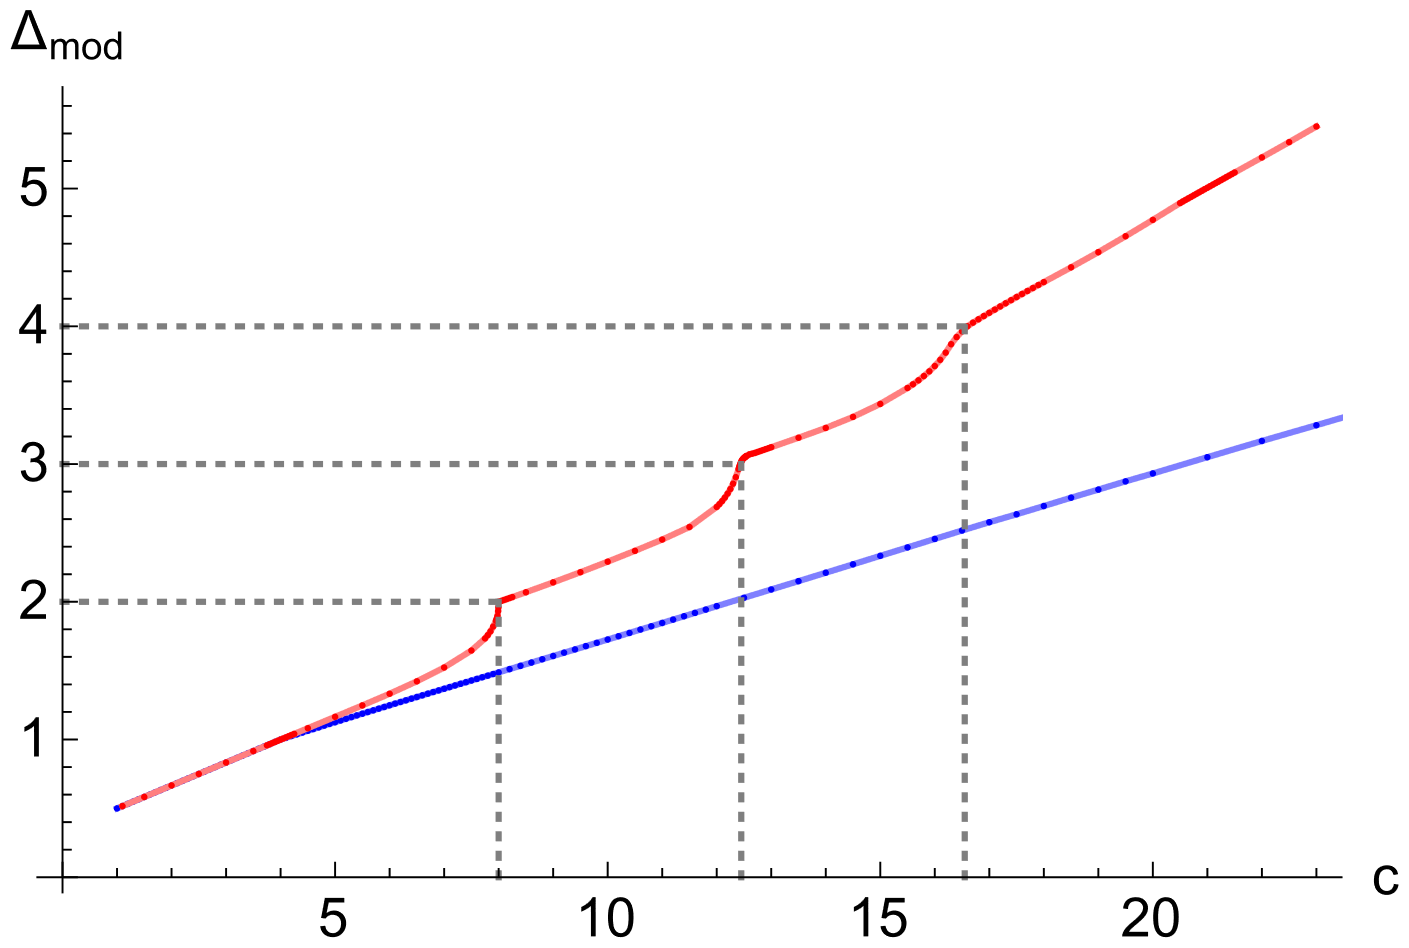
\includegraphics[width=0.85\textwidth]{figures/fig12.png}
  \caption{最轻标量算符维数的模界 $\Delta_{\mathrm{mod}}^{s=0}$（红色）作为中心荷 $c$ 的函数，与全自旋维数间隙界 $\Delta_{\mathrm{mod}}$（蓝色）作比较 \cite{r58}。（原文 p.35，图 12）}
  \label{fig:12}
\end{figure}

按定义，$c\le4$ 时 $\Delta_{\mathrm{mod}}^{s=0}(c)$ 与 $\Delta_{\mathrm{mod}}(c)$ 重合，此处界不超过 $1$。$c>4$ 时 $\Delta_{\mathrm{mod}}^{s=0}(c)$ 严格大于 $\Delta_{\mathrm{mod}}(c)$，并在 $c=25$ 处发散。数值结果还显示出若干有趣特征。界 $\Delta_{\mathrm{mod}}^{s=0}(c)$ 在 $c=8$ 处有一个折点，该处界等于 $2$。这意味着中心荷 $c<8$ 的一切 CFT 都必须含一个非平凡的相关标量 Virasoro 原初场。还可看到，在特殊值 $c=1,2,\frac{14}{5},4,8$ 处，标量间隙界 $\Delta_{\mathrm{mod}}^{s=0}$ 被规范群为 $SU(2)$、$SU(3)$、$G_2$、$SO(8)$、$E_8$ 的能级 $1$ WZW 模型饱和。
% [Tutor Note: $c=8$ 处界等于 $2$ 的物理含义要紧扣“相关”二字：$\Delta_{\mathrm{mod}}^{s=0}<2$ 表示谱中必有标量原初场维数小于 $2$，即相关算符。$c>8$ 后界超过 $2$，就不再强制相关标量存在，故 $c<8$ 的说法是严格的。五个饱和点是 $SU(2)_1$（$c=1$）、$SU(3)_1$（$c=2$）、$(G_2)_1$（$c=\frac{14}{5}$）、$SO(8)_1$（$c=4$）、$(E_8)_1$（$c=8$），它们都是自对偶的能级 $1$ WZW 模型。]

我们也可以束缚间隙处的标量简并度，只需换一个优化问题。考虑形如 \eqref{eq:5-2} 的线性泛函，并作归一化
\begin{equation}
  \label{eq:5-9}
  \alpha[\chi_0\bar\chi_0]=-1 .
\end{equation}
现在对第一个标量原初场 $h=\tilde h=\frac12\Delta_*$，求 $\alpha[\chi_h\bar\chi_{\tilde h}]$ 的极大值，约束为
\begin{equation}
  \label{eq:5-10}
  \begin{aligned}
  &\alpha[\chi_h\bar\chi_{\tilde h}]\ge0,\qquad h=\tilde h\ge\tfrac12\Delta_*,\\
  &\text{or}\quad h\ne\tilde h,\ h,\tilde h\ge0,\ h-\tilde h\in\mathbb{Z} .
  \end{aligned}
\end{equation}
设已找到这样的线性泛函 $\alpha_*$，把它代入模交叉方程，得
\begin{equation}
  \label{eq:5-11}
  \begin{aligned}
  0&=\alpha_*\Bigl[\chi_0\bar\chi_0+d_{\mathrm{gap}}\,\chi_{\frac{\Delta_0}{2}}\bar\chi_{\frac{\Delta_0}{2}}
  +\sum_{\mathrm{rest}}\chi_h\bar\chi_{\tilde h}\Bigr]\\
  &\ge-1+d_{\mathrm{gap}}\,\alpha_*\Bigl[\chi_{\frac{\Delta_0}{2}}\bar\chi_{\frac{\Delta_0}{2}}\Bigr],
  \end{aligned}
\end{equation}
其中 $d_{\mathrm{gap}}$ 是维数 $\Delta_0$ 处的标量简并度。于是 $\bigl(\alpha_*[\chi_{\frac{\Delta_0}{2}}\bar\chi_{\frac{\Delta_0}{2}}]\bigr)^{-1}$ 给出 $d_{\mathrm{gap}}$ 的严格上界。当然，$\Delta_0$ 不应超过 $\Delta_{\mathrm{mod}}^{s=0}$。图~\ref{fig:13} 给出 $\Delta_0=\Delta_{\mathrm{mod}}^{s=0}$ 时 $d_{\mathrm{gap}}$ 的上界在一段 $c$ 范围内的数值结果。

\begin{figure}[htbp]
  \centering
  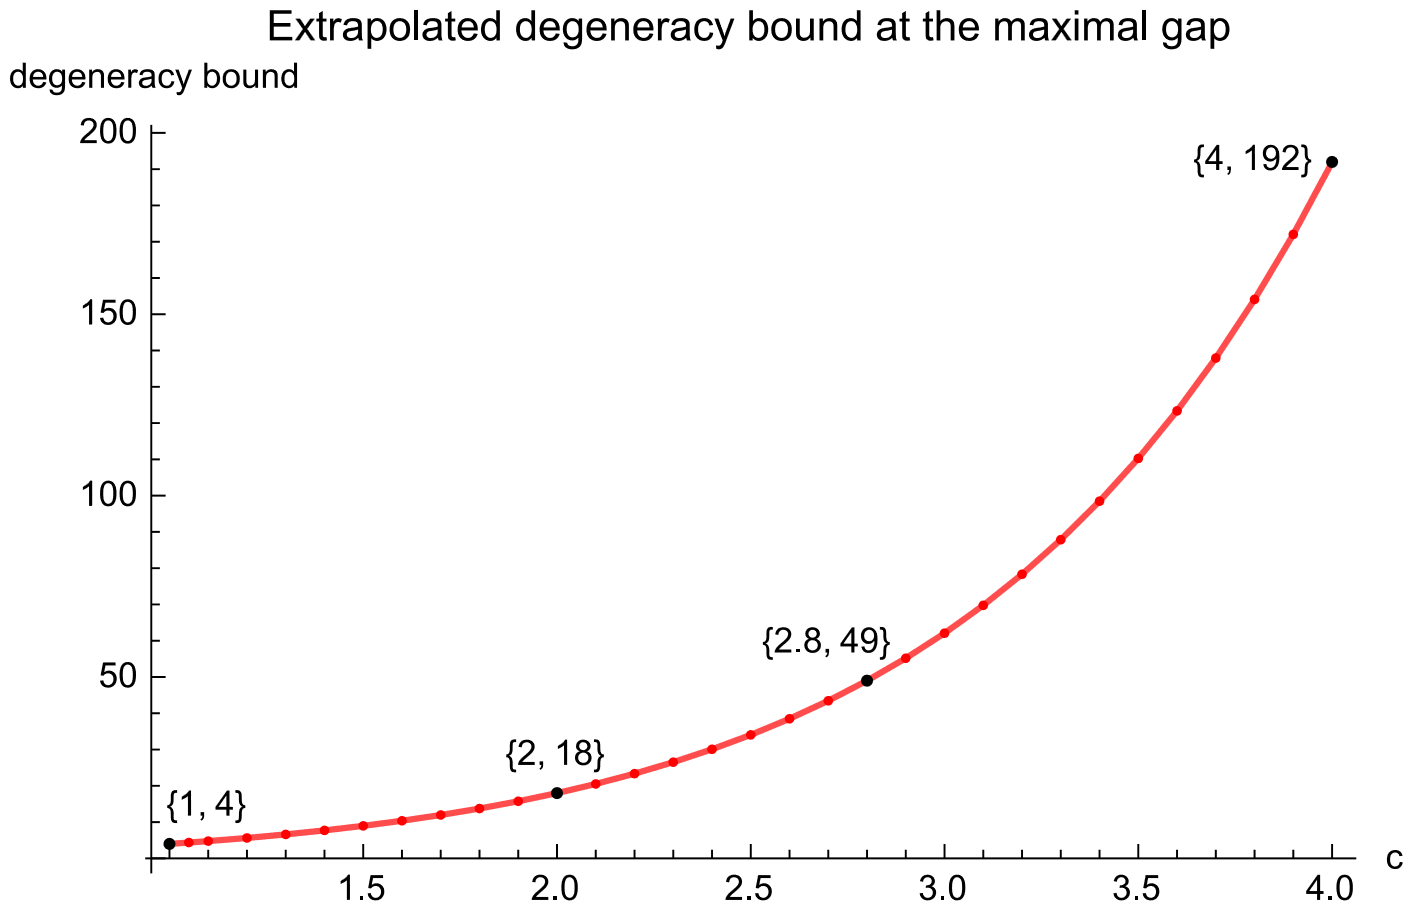
\includegraphics[width=0.85\textwidth]{figures/fig13.png}
  \caption{$\Delta_{\mathrm{mod}}^{s=0}(c)$ 处标量简并度的上界，$1\le c\le4$。黑点对应 $SU(2)_1$、$SU(3)_1$、$(G_2)_1$ 与 $SO(8)_1$ WZW 模型，简并度界在这些点上饱和 \cite{r58}。（原文 p.36，图 13）}
  \label{fig:13}
\end{figure}

\begin{figure}[htbp]
  \centering
  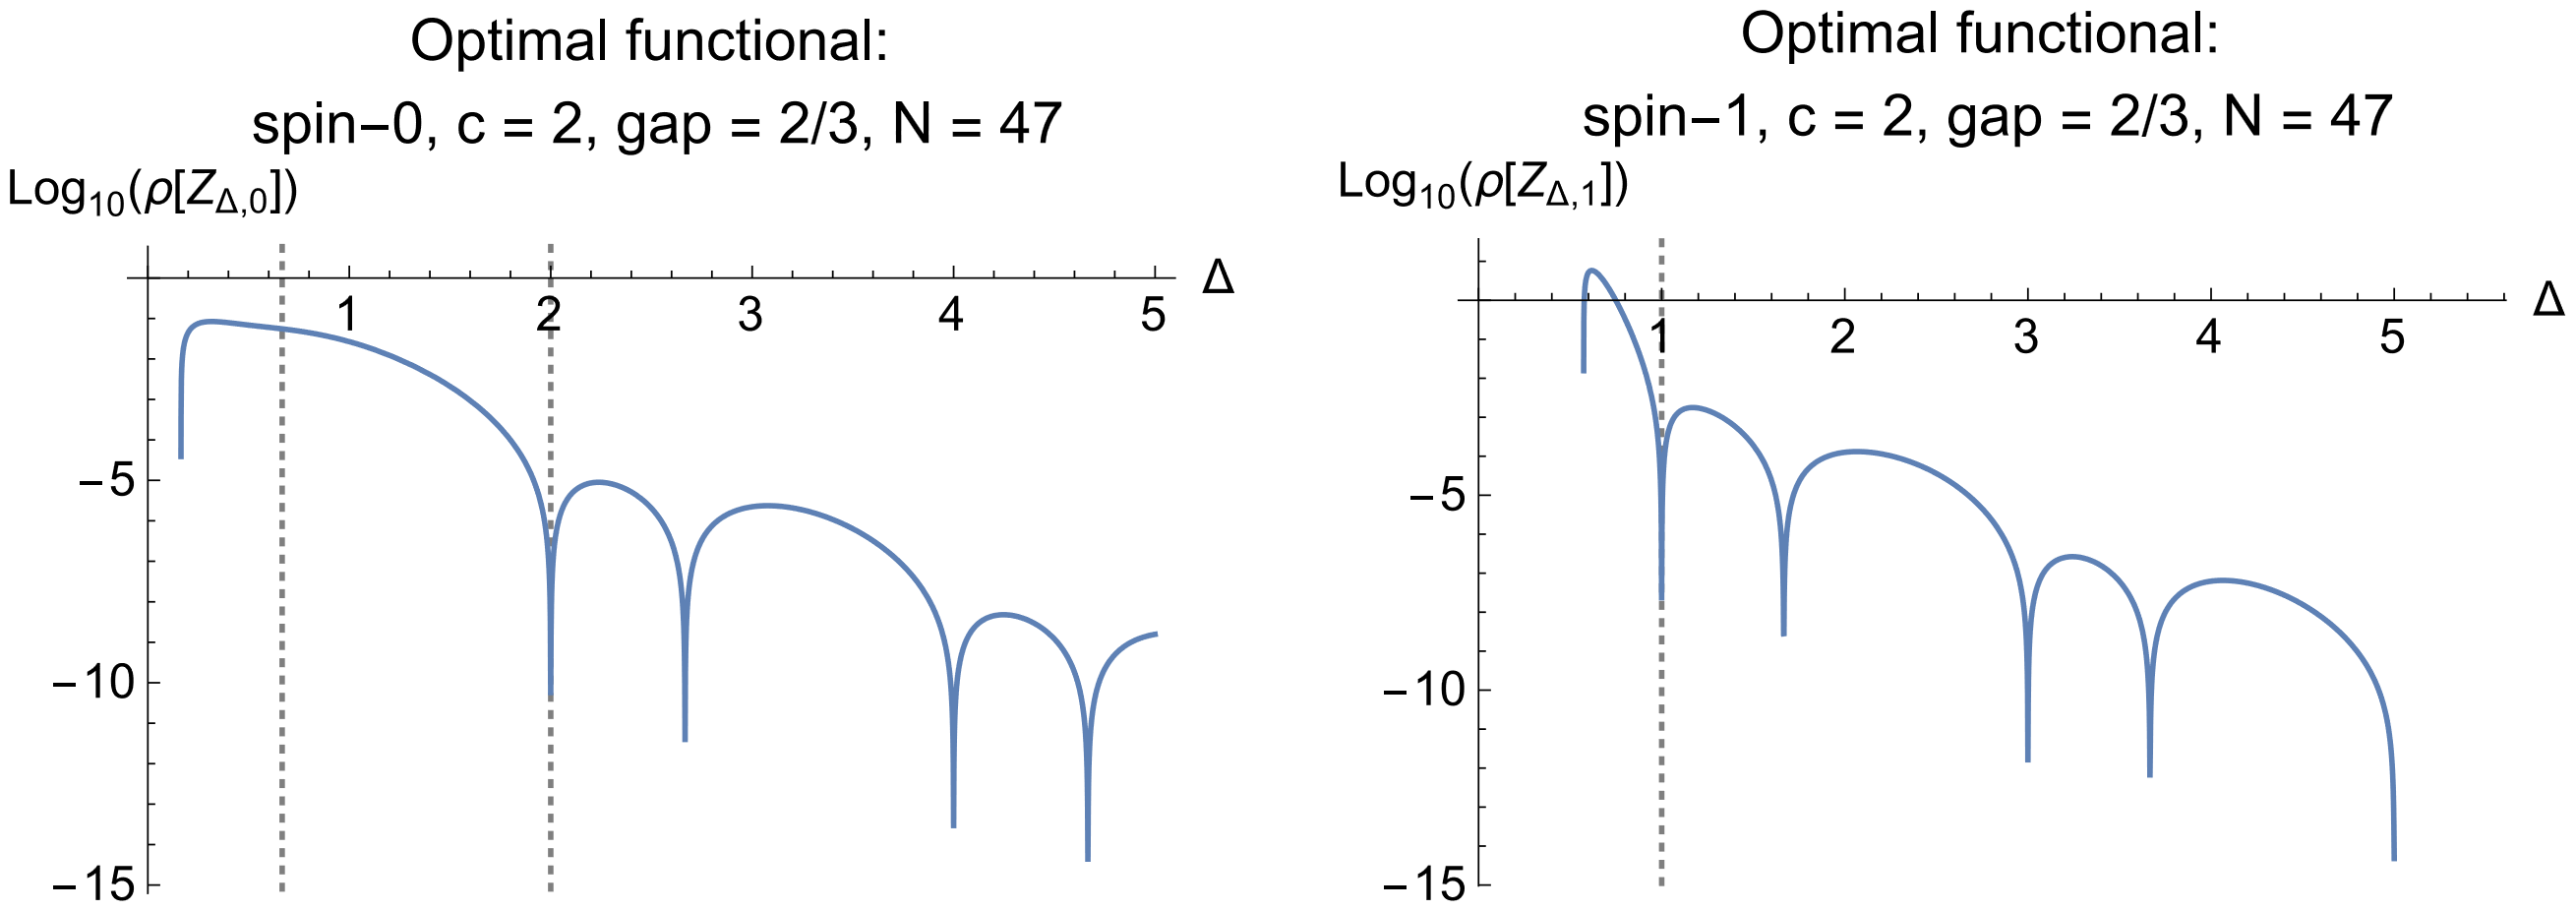
\includegraphics[width=0.85\textwidth]{figures/fig14.png}
  \caption{间隙处算符简并度取极大、且 $c=2$ 处维数间隙界被饱和时，最优泛函作用在自旋 $0$ 与自旋 $1$ 特征标上的对数图。竖直虚线标出间隙，以及自旋 $0$ 情形下的边缘标量原初场与自旋 $1$ 情形下的守恒自旋 $1$ 流 \cite{r58}。（原文 p.36，图 14）}
  \label{fig:14}
\end{figure}
% [Tutor Note: 图 14 两个面板的横轴都是 $\Delta$，纵轴是 $\log_{10}\rho[\cdots]$，即泛函在对应特征标上的取值取对数。读数要点：曲线在每个原初场维数处出现向下的尖峰（即泛函的零点）；左图第二条竖直虚线在 $\Delta=2$，对应边缘标量原初场，右图虚线在 $\Delta=1$，对应守恒自旋 $1$ 流。$c=2$ 的 $SU(3)_1$ 正是标量间隙界与简并度界同时饱和的模型，故其零点位置与 $SU(3)_1$ 的谱结构对应。]

若某个 CFT 恰好饱和了 $d_{\mathrm{gap}}$ 的界，则谱中其余部分的 $(h,\tilde h)$ 必须满足 $\alpha_*[\chi_h\bar\chi_{\tilde h}]=0$。换言之，原初场谱的其余部分落在 $\alpha_*[\chi_h\bar\chi_{\tilde h}]$ 作为 $(h,\tilde h)$ 的函数的零点集内。这就是“极值泛函方法” \cite{r59,r60}。只要某个特征标或共形块展开的系数已知、或被猜想为在所关心的 CFT 上取极大，该方法就能用于各种自举分析。

$c=2$ 的一个例子见图~\ref{fig:14}：使间隙 $\Delta_0=\frac23$ 最大的极值泛函 $\alpha_*$，在自旋 $0$ 与自旋 $1$ 特征标上的零点，与相应自旋的 $SU(3)$ WZW 模型在标量间隙之上的谱吻合。

\subsection{束缚谱函数}\label{sec:5-2}

本节转向谱函数方法。它从交叉方程中提取的不仅是算符谱间隙的界，还包括整个谱上算符贡献的界 \cite{r61}。

设四个全同标量原初场的维数为 $\Delta_\phi$。其四点函数 $g(z,\bar z)=\langle\phi(0)\phi(z,\bar z)\phi(1)\phi'(\infty)\rangle$ 的共形块分解为
\begin{equation}
  \label{eq:5-12}
  g(z,\bar z)=\sum_{h,\tilde h}C^2_{h,\tilde h}\,\mathcal{F}_h(z)\overline{\mathcal{F}}_{\tilde h}(\bar z),
\end{equation}
% [Tutor Note: 原文第四个算符写作 $\phi'(\infty)$，带一撇；按“四个全同标量原初场”的上下文，通常应读作 $\phi(\infty)$。此处照原文排，核对时不必据此改动 $C^2_{h,\tilde h}$ 的定义。]
其中 $C^2_{h,\tilde h}$ 表示 $\phi\phi$ OPE 中权重为 $(h,\tilde h)$ 的原初场的 OPE 系数平方和，$\mathcal{F}_h(z)$ 是内权重为 $h$ 的 Virasoro 共形块（这里略去了对 $\phi$ 的权重与中心荷 $c$ 的显式依赖）。交叉方程取形式
\begin{equation}
  \label{eq:5-13}
  \sum_{h,\tilde h}C^2_{h,\tilde h}\bigl[\mathcal{F}_h(z)\overline{\mathcal{F}}_{\tilde h}(\bar z)
  -\mathcal{F}_h(1-z)\overline{\mathcal{F}}_{\tilde h}(1-\bar z)\bigr]=0,
\end{equation}
或写成 $F^{m,n}(h,\tilde h)\equiv\partial_z^m\partial_{\bar z}^n[\mathcal{F}_h(z)\overline{\mathcal{F}}_{\tilde h}(\bar z)]_{z=\bar z=\frac12}$ 的形式：
\begin{equation}
  \label{eq:5-14}
  \sum_{h,\tilde h}C^2_{h,\tilde h}F^{m,n}(h,\tilde h)=0,\qquad m,n\ge0,\ m+n\ \text{odd} .
\end{equation}
% [Tutor Note: 与 (5.2) 同理，(5.14) 只取 $m+n$ 为奇数的项。设 $u=z-\frac12$，则 $z\to1-z$ 就是 $u\to-u$；交叉方程在 $z=\bar z=\frac12$ 附近作 Taylor 展开时，$\mathcal{F}_h(z)\overline{\mathcal{F}}_{\tilde h}(\bar z)-\mathcal{F}_h(1-z)\overline{\mathcal{F}}_{\tilde h}(1-\bar z)$ 的偶阶项自动抵消，只剩奇数阶。故 $F^{m,n}$ 只需对 $m+n$ 奇数取值。]

注意共形块自身在 $z=\bar z=\frac12$ 处恒为正，即 $F^{0,0}(h,\tilde h)>0$（$h,\tilde h\ge0$）。定义谱函数
\begin{equation}
  \label{eq:5-15}
  f(\Delta_*)=\frac{\sum_{h+\tilde h<\Delta_*}C^2_{h,\tilde h}\,
  \mathcal{F}_h(\frac12)\overline{\mathcal{F}}_{\tilde h}(\frac12)}
  {g(\frac12,\frac12)} .
\end{equation}
按定义，幺正 CFT 中全同算符四点关联函数的谱函数是单调不减的，取值介于 $0$ 与 $1$ 之间。它度量维数不超过 $\Delta_*$ 的算符对关联函数的贡献。

利用交叉方程，可以给出 $f(\Delta_*)$ 作为 $\Delta_*$ 的函数的非平凡上下界。为此考虑不等式
\begin{equation}
  \label{eq:5-16}
  \theta(\Delta_*-\Delta)-y_{0,0}-\sum_{m+n\ \text{odd}}y_{m,n}
  \frac{F^{m,n}(h,\tilde h)}{F^{0,0}(h,\tilde h)}\ge0,
  \qquad\forall (h,\tilde h)\in\mathcal{S},
\end{equation}
其中 $\mathcal{S}$ 是 $\phi\phi$ OPE 中出现算符的假想谱，$y_{m,n}\in\mathbb{R}$。对任一给定的 $\Delta_*$，若能找到一组 $y_{m,n}$，使 \eqref{eq:5-16} 对所有满足 $\mathcal{S}$ 上假设的权重 $(h,\tilde h)$ 同时成立，则用 $C^2_{h,\tilde h}F^{0,0}(h,\tilde h)$ 乘 \eqref{eq:5-16}、对 OPE 中的算符求和，并利用交叉方程，得
\begin{equation}
  \label{eq:5-17}
  \sum_{h,\tilde h}C_{h,\tilde h}\bigl[\Theta(\Delta_*-\Delta)-y_{0,0}\bigr]F^{0,0}(h,\tilde h)
  =g\bigl(\tfrac12,\tfrac12\bigr)\bigl(f(\Delta_*)-y_{0,0}\bigr)\ge0 .
\end{equation}
% [Tutor Note: 原文 (5.17) 的求和号前写的是 $C_{h,\tilde h}$，没有平方。按 (5.12) 与交叉方程的求和权重，这里应为 $C^2_{h,\tilde h}$；否则等号右边无法凑出 $g(\frac12,\frac12)f(\Delta_*)$。此处照原文排，属原文笔误。另外 (5.16) 与 (5.17) 里的小写 $\theta$ 与大写 $\Theta$ 是同一阶梯函数，只是原文大小写不一致。]

于是 $y_{0,0}$ 是 $f(\Delta_*)$ 的严格下界。在 \eqref{eq:5-16} 的约束下极大化 $y_{0,0}$，就得到 $f(\Delta_*)$ 的最优下界。数值上用半正定规划求解；作截断 $m+n\le N$ 后得到谱函数的下界，记作 $f_-^{(N)}(\Delta_*)$。同理，在 \eqref{eq:5-16} 的反向不等式约束下极小化 $y_{0,0}$，得到上界 $f_+^{(N)}(\Delta_*)$。

作为玩具例子，取 $N=1$，即只用一阶导数。若用 $z^{-2h_\phi+h}$ 近似 $\mathcal{F}(h;z)$（有时称作“标度块”），则可写 $F^{1,0}/F^{0,0}\approx2(-2h_\phi+h)$，并推出谱函数的下界
\begin{equation}
  \label{eq:5-18}
  y_{0,0}(x)\approx1-\frac{2\Delta_\phi}{x} .
\end{equation}
这个结果当然只是近似，但与 \eqref{eq:5-16} 给出的精确界定性相似。不过它在权重大时相当弱；我们早已知道，高维原初场的尾部贡献必定指数压低。

\begin{figure}[htbp]
  \centering
  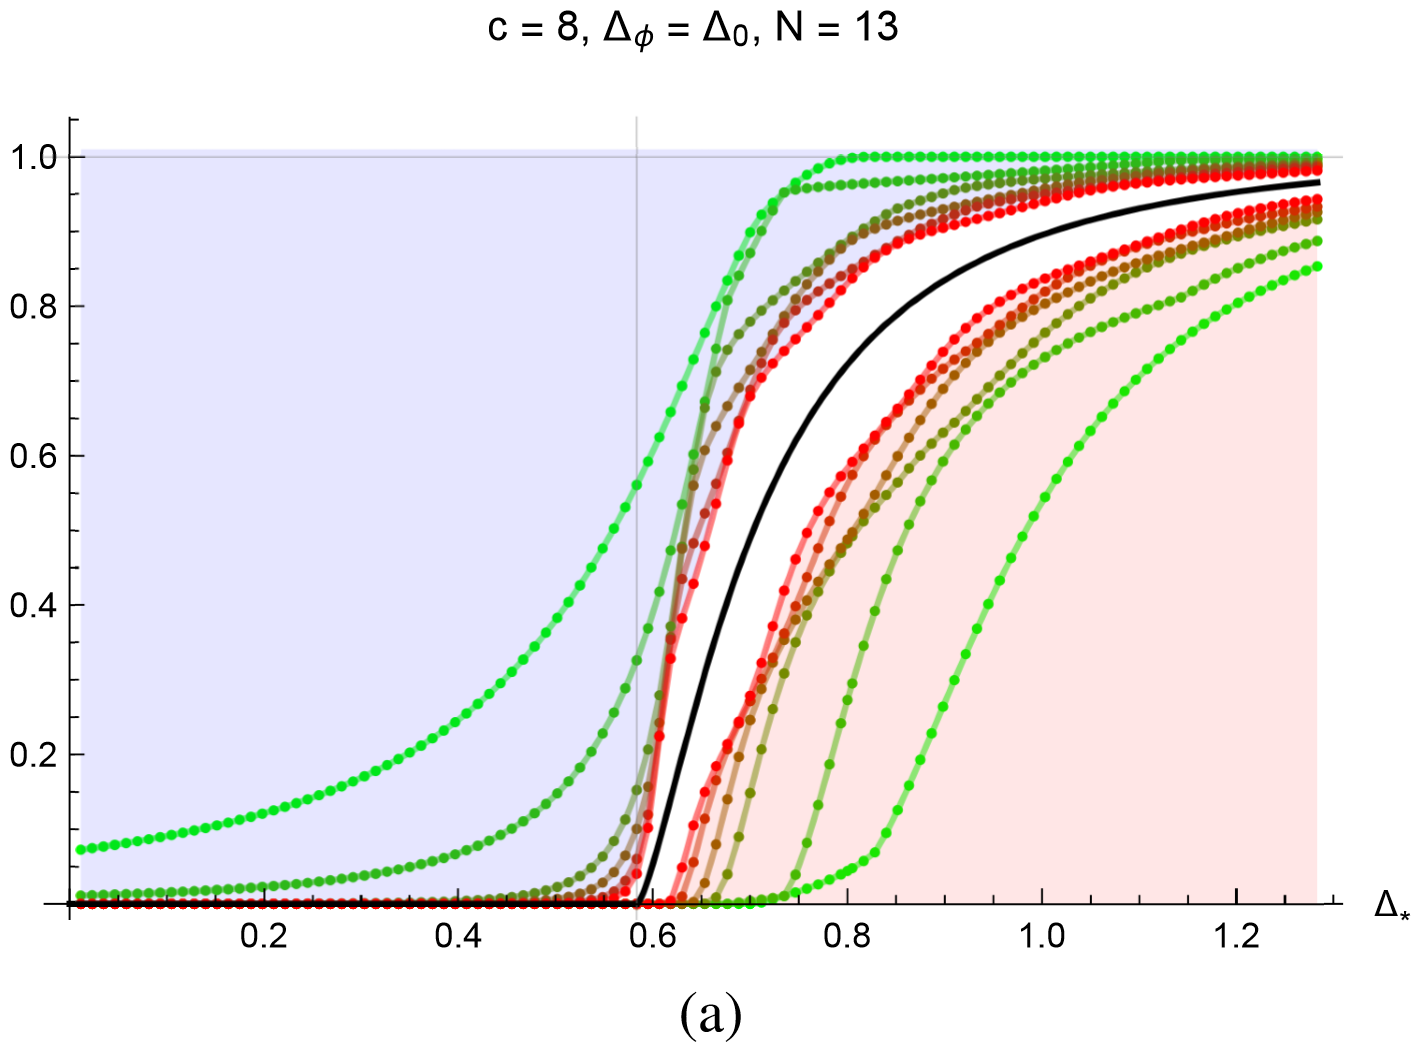
\includegraphics[width=0.85\textwidth]{figures/fig15.png}
  \caption{导数阶 $N$ 递增的线性泛函（由绿到红）给出的谱函数上下界，假设只有标量原初场，取 $c=8$、$\Delta_\phi=\frac{7}{12}$。阴影区被排除，黑线为 Liouville 理论对应的谱函数 \cite{r61}。（原文 p.38，图 15）}
  \label{fig:15}
\end{figure}
% [Tutor Note: (5.18) 里的 $x$ 就是 $\Delta_*$，与 (5.16) 的自变量一致；$1-2\Delta_\phi/x$ 在 $x\gg\Delta_\phi$ 时趋于 $1$，但精确界在 $x\to\infty$ 时会更慢地趋于 $1$。图中绿线到红线对应 $N$ 增大，允许窗口逐级收窄，把黑线（Liouville 谱函数）夹在中间；左侧蓝色与右侧红色阴影区都是被界排除的区域。]

下面考察一个只含标量 Virasoro 原初场（即没有非零自旋原初场）的 $c>1$ 的 CFT 中 $\langle\phi\phi\phi\phi\rangle$ 的谱函数界。我们已经看到，这一假设与模不变性结合，意味着该 CFT 是非紧致的、维数间隙为 $\frac{c-1}{12}$，且其谱密度等于 Liouville CFT 的谱密度。现在若已知谱函数 $f(\Delta_*)$，对 $\Delta_*$ 求导即可还原全部 OPE 系数。

截止到 $N=13$ 的 $f_\pm^{(N)}(\Delta_*)$ 数值结果示例见图~\ref{fig:15}。这些界夹出一个允许的窗口，Liouville 谱函数落在其中。上下界在 $N\to\infty$ 极限下有可能收敛，但数值上难以看出，因为截断阶 $N$ 增高时计算这些界变得非常耗时。

若假定 $N=\infty$ 时上下界重合，就可以直接求解等式
\begin{equation}
  \label{eq:5-19}
  \theta(\Delta_*-\Delta)=y_{0,0}+\sum_{m+n\ \text{odd}}y_{m,n}\,
  \frac{F^{m,n}\bigl(\frac{\Delta}{2},\frac{\Delta}{2}\bigr)}
  {F^{0,0}\bigl(\frac{\Delta}{2},\frac{\Delta}{2}\bigr)},
  \qquad\forall\Delta\ge0 .
\end{equation}
对一切 $\Delta_*\ge0$ 都有解，这等价于 $p_{m,n}(\Delta)=\frac{F^{m,n}(\frac{\Delta}{2},\frac{\Delta}{2})}{F^{0,0}(\frac{\Delta}{2},\frac{\Delta}{2})}$ 作为 $\Delta$ 的函数在正实轴上构成一组完备基，相应的 Hilbert 空间内积为
\begin{equation}
  \label{eq:5-20}
  \langle x,y\rangle=\int_0^\infty x^*(\Delta)\,y(\Delta)\,\mu(\Delta)\,d\Delta ,
\end{equation}
其中 $\mu(\Delta)$ 是某个合适的测度因子。设 $\rho(\Delta)$ 为谱密度，则四点函数在 $z=\bar z=\frac12$ 处的共形块分解取形式 $\int d\Delta\,\rho(\Delta)\,C_\Delta^2F^{0,0}(\frac{\Delta}{2},\frac{\Delta}{2})$。我们想定义矢量 $v(\Delta)=\frac{\rho(\Delta)C_\Delta^2F^{0,0}(\frac{\Delta}{2},\frac{\Delta}{2})}{g(\frac12,\frac12)\mu(\Delta)}$，使之满足
\begin{equation}
  \label{eq:5-21}
  \begin{aligned}
  \langle v,p_{0,0}\rangle&=1,\\
  \langle v,p_{m,n}\rangle&=0,\qquad m,n\ge0,\ m+n\ \text{odd} .
  \end{aligned}
\end{equation}

\begin{figure}[htbp]
  \centering
  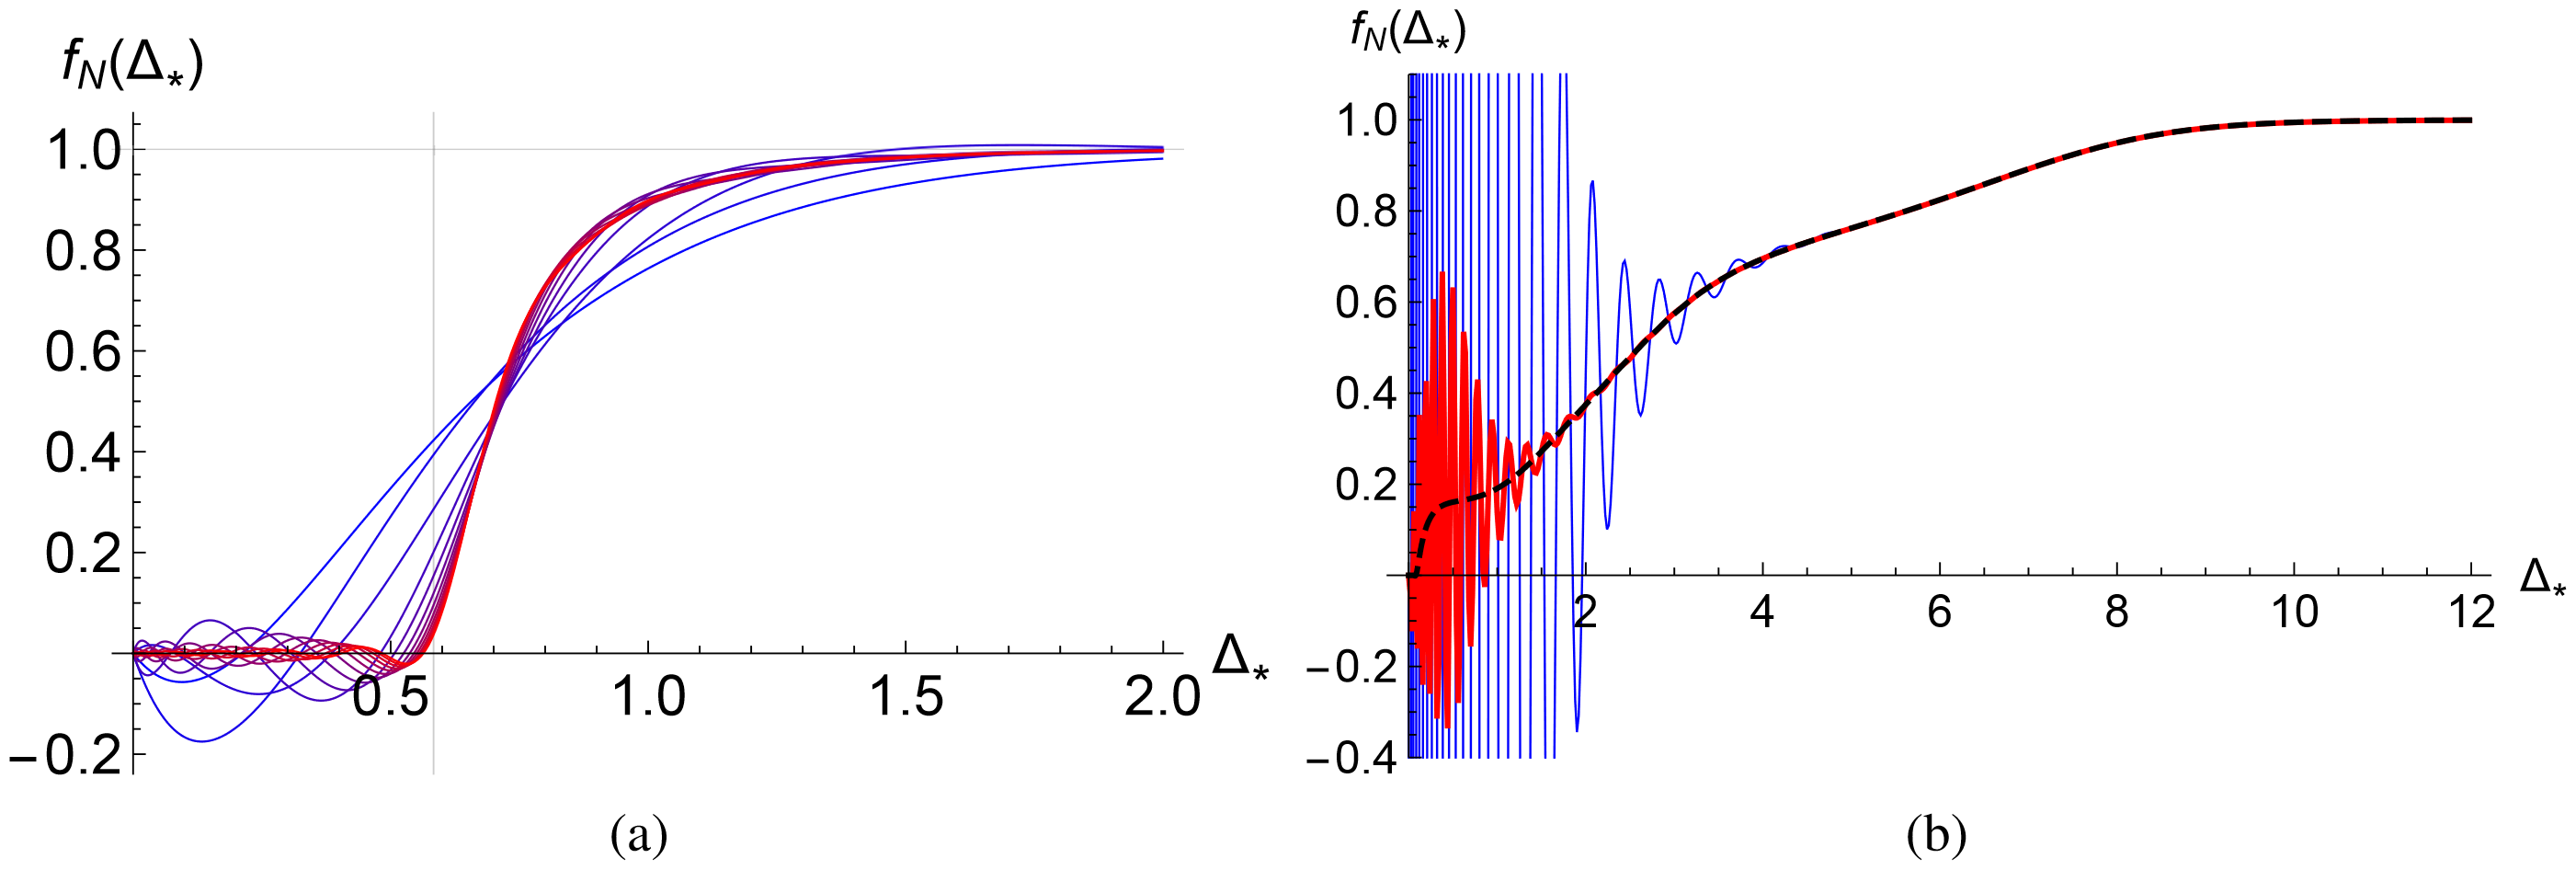
\includegraphics[width=0.85\textwidth]{figures/fig16.png}
  \caption{(a) $c=8$、$\Delta_\phi=\frac{7}{12}$ 时 $f_N(\Delta_*)$ 的图，$N$ 从 $N=1$（蓝）取到 $N=25$（红），步长为 $2$。(b) $c=2$、$\Delta_\phi=\frac{55}{12}$ 时 $f_N(\Delta_*)$（$N=27$ 为蓝色实线，$N=33$ 为红色实线）与精确 DOZZ 谱函数（黑色虚线）的比较。图取自 \cite{r61}。（原文 p.39，图 16）}
  \label{fig:16}
\end{figure}

% [Tutor Note: 原文图 16 (b) 的图注印作 $\Delta_\phi=\frac{55}{12}$（$c=2$）；同图 (a) 的 $7/12=(c-1)/12$，而 $55/12$ 与该关系不符，疑为 $5/12$ 之误或作者另取的参数。译文照原样排，引用该参数时请核对底本。]

测度因子 $\mu(\Delta)$ 的取法应保证内积 $\langle v,v\rangle$ 与 $\langle p_{m,n},p_{m,n}\rangle$ 在 $\Delta$ 上都是收敛积分。回忆 Virasoro 共形块在 $\Delta$ 大时按 $(16q)^\Delta$ 增长（$q$ 为椭圆 nome），OPE 的收敛要求 $\rho(\Delta)C_\Delta^2$ 至少按 $16^{-\Delta}$ 衰减，于是 $\mu(\Delta)v(\Delta)$ 至少按 $e^{-\pi\Delta}$ 衰减。$p_{m,n}(\Delta)$ 按 $\Delta$ 的多项式增长。因此取 $\mu(\Delta)\sim e^{-\lambda\Delta}$，只要 $0<\lambda<2\pi$，即可保证 $\langle v,v\rangle$ 与 $\langle p_{m,n},p_{m,n}\rangle$ 都收敛。实践中取 $\lambda=\pi$。现在取 $v$ 与 \eqref{eq:5-19} 的内积，就得到谱函数
\begin{equation}
  \label{eq:5-22}
  f(\Delta_*)=\langle v,\theta(\Delta_*-\Delta)\rangle .
\end{equation}
% [Tutor Note: 这里省了半步：把 (5.19) 与 $v$ 作内积，右边得 $y_{0,0}\langle v,p_{0,0}\rangle+\sum y_{m,n}\langle v,p_{m,n}\rangle=y_{0,0}$，故 (5.22) 等于说 $y_{0,0}$ 的最优值就是 $f(\Delta_*)$，这正是上下界在 $N=\infty$ 重合的假设所保证的。另注意 $e^{-\pi\Delta}$ 的来源：$z=\bar z=\frac12$ 时椭圆 nome 满足 $q=e^{-\pi K(1-z)/K(z)}=e^{-\pi}$，故 $(16q)^{\Delta}\cdot16^{-\Delta}=e^{-\pi\Delta}$；取 $\lambda<2\pi$ 即要求测度比 $v$ 衰减得更快。]
% [Tutor Note: 补充说明 (5.20) 一式的用意：它把交叉方程的解存在性翻译成函数系 $\{p_{m,n}\}$ 的完备性；原文说“the existence of solution for all $\Delta_*\ge0$ amounts to the completeness”，依据就是 $y_{m,n}$ 与 $\Delta_*$ 无关、而 $\theta(\Delta_*-\Delta)$ 作为 $\Delta$ 的函数必须能在此基下展开。这是标准的矩问题（Hamburger 型）论证。]

% ---------------------------------------------------------------------------
% 本节（5.2）在原书 p.39 末并未结束，续译见后续片段。
% ---------------------------------------------------------------------------

